\documentclass[10pt]{article}

% Set paper size and margins
\usepackage[a4paper, width=150mm, top=40mm, bottom=50mm, headsep=10mm, footskip=25mm]{geometry}

% Set line spacing
\renewcommand{\baselinestretch}{1.5}


\usepackage{graphicx}
\usepackage[table]{xcolor}
\usepackage{longtable}
\usepackage{amsfonts}

\bibliographystyle{unsrt2authabbrvpp}
\begin{document}

% Title page
\begin{titlepage}
%	From model start & Remote learning & 0.1 \\
\centering
\vspace*{3cm}
\huge
\textbf{Methods used in AuTuMN modelling of the COVID-19 epidemic in Sri Lanka}
\vspace{0.5cm}
\end{titlepage}

% Table of contents
\clearpage
{
    \sffamily
    \tableofcontents
}
\clearpage

% This file describes the general structure of some of our tb_dynamics models.

\section{Model Structure}

\subsection{General features}

We use a deterministic compartmental model including six types of compartments that represent 
different states of infection and disease. The model uses the same conceptual approach and similar 
assumptions to previously published models \cite{trauer-2017, ragonnet-2019, ragonnet-2021, ragonnet-2022}. 
Here we describe the model structure without treatment compartment and related factors. 
\newline
A susceptible compartment (S) is used to represent individuals who have 
never been infected with \emph{Mycobacterium tuberculosis (M.tb)}. Latent TB infection (LTBI) is modelled 
using two successive compartments: early latent (E) and late latent (L) to capture the declining risk of 
disease progression over time from infection \cite{ragonnet-2017}. The active disease compartment (I) represents 
individuals who have progressed to the active stage of TB disease. Diseased individuals who recover 
through self-cure progress directly to the recovered compartment (R).
\newline
Non-TB-related mortality is modelled by applying death rates to all model compartments. In addition, 
disease-specific mortality is implemented by applying increased mortality rates to the active disease 
compartments (I).
\newline
Reinfection occurs in the model in two different ways. First, latently infected individuals may be 
reinfected, with this process modelled using a flow from the late latent (L) to the early latent 
compartment (E). Second, individuals who have recovered from TB disease may be reinfected and 
return to the early latent compartment. The structure of our model allows for differential risk of 
infection for the currently and previously infected individuals, compared to the infection-naive 
individuals.
\begin{figure}[!htp]
    \vspace*{-1cm}
    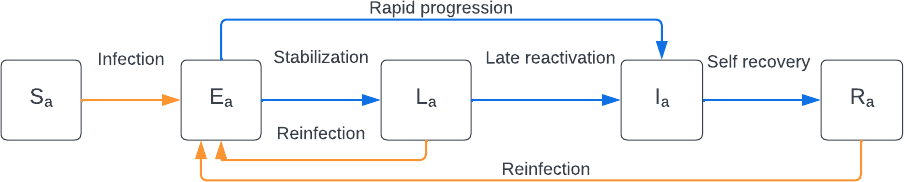
\includegraphics[width=\textwidth,height=\textheight,keepaspectratio]{images/model.png}
    \caption{Illustration of the model structure. 
    Boxes represent the different compartments types: susceptible (S), early latent (E), late latent (L), infectious (I), and recovered (R).
    The subscript indicates that compartments are stratified by age (a).}
    \label{fig:model}
\end{figure}

\subsection{Stratification by age}
The model is stratified using five categories: 0-4, 5-14, 15-34, 35-49 and 50+ years old. We assume 
heterogeneous mixing by age using an age-specific contact rate matrix. Since no local estimates of 
contact patterns by age were available for the Marshall Islands, we used a contact survey conducted in 
the Fijian population and adjusted the estimates to account for age distribution differences between
the two countries.


\subsection{Model stratification}
% Note that this will vary for every application, so will need to be edited - not sure of how best to manage this:
All compartments of the base compartmental structure were stratified by age, location and organ status:\linebreak
Age
\begin{itemize}
    \item Zero to 14 years
    \item 15 to 24 years
    \item 25 to 49 years
    \item 50 to 69 years
    \item 70 years and above
\end{itemize}
Location
\begin{itemize}
    \item South Tarawa
    \item Other location
\end{itemize}
Organ status
\begin{itemize}
    \item Pulmonary smear-posivtive
    \item Pulmonary smear-negative
    \item Extrapulmonary
\end{itemize}

\section{Clinical stratification} \label{clin}
% Note that this file describes only one implementation of the clinical stratification possible in the sm_sir code
The ``clinical" stratification acts by replicating each of the two age-stratified sequential compartments representing infectious COVID-19 into three categories.
The three clinical categories are:
\begin{enumerate}
    \item Asymptomatic persons
    \item Symptomatic persons who are never notified as cases
    \item Symptomatic persons who are successfully detected and notified
\end{enumerate}
For each age category, a proportion of new active infections are assumed to remain asymptomatic throughout their infectious period (specified in Table \ref{tab:age_params}).
This proportion remains fixed over time throughout a model run.
It is assumed that asymptomatic persons are never detected and so do not contribute to notifications.
The remaining proportion constitutes the second and third categories, comprising all persons developing symptomatic COVID-19 during their infectious period.
The proportion of these symptomatic persons who progress to the third category varies with time and is described under the section on case detection (Section \ref{cdr}).
\begin{figure}[ht]
    \begin{center}
    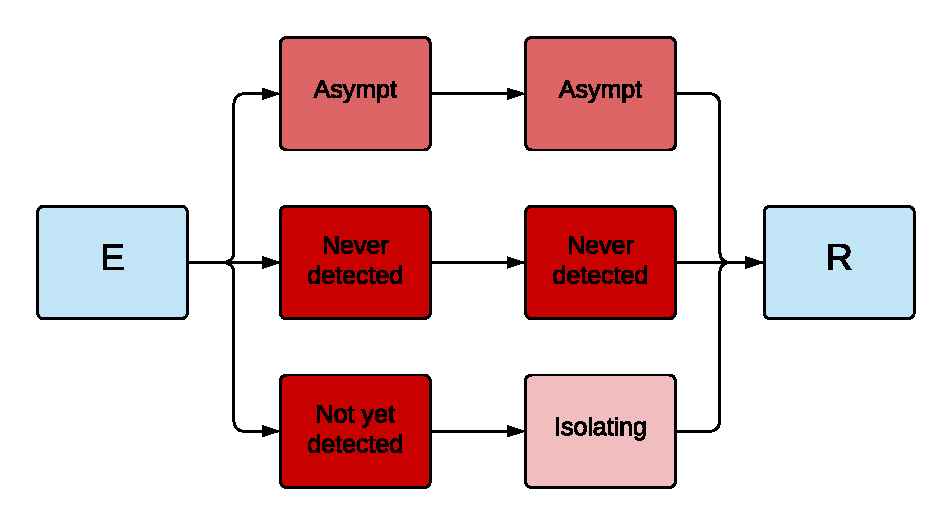
\includegraphics[width=0.7\textwidth]{../../tex_descriptions/models/sm_sir/stratifications/clinical_strat.pdf}
    \end{center}
    \caption{Illustration of the clinical stratification. \small Depth of red shading of compartment qualitatively indicates infectiousness.}
    \label{fig:seeiir}
\end{figure}

The model was stratified by ``strain'' to simulate the emergence of multiple variants of concern (VoC).
This approach explicitly represents multiple competing strains, each with an independent force of infection calculation.
We assumed that VoCs can have different levels of transmissibility, incubation period and disease severity 
(hospitalisation and death risks) compared to the ancestral COVID-19 strain. In addition, VoCs were assumed to escape 
immunity partially for both vaccination- and infection-related immunity. 

We assumed that individuals previously infected with the wild-type strain could only be reinfected with the delta or 
omicron strains. However, such individuals have a reduced risk of infection with these variants compared to 
infection-naive individuals (82\% and 45\% reduction for delta and omicron, respectively) \cite{stein2023}.
We assumed that individuals previously infected with the delta variant could only be reinfected with the omicron variant, 
with an infection risk reduced by 45\% compared to infection-naive individuals \cite{stein2023}. 
The other parameters used to represent strain-specific characteristics are presented in Table \ref{param_table}.

Seeding of each new strain into the model was achieved through the importation of a small number (10 per million population) of new infectious persons with the relevant strain into the model.
The seeding process was implemented over a ten-day period, with the start of this period extracted from the GISAID database for each country \cite{gisaid2023}. 
We considered a strain (either Delta or Omicron) to have emerged when, during a single week in GISAID, at least two cases of that strain were reported, and these cases accounted for at least 1\% of all reported cases during that week.

\section{Vaccination}

\subsection{Model structure}
In this application we introduced separate strata to the model for vaccinated an unvaccinated individuals.
All model compartments are replicated into three categories:

\begin{itemize}
	\item Unvaccinated persons
	\item Persons who have only received one dose of vaccination
	\item Persons who have received two doses of vaccination (i.e. the full course)
\end{itemize}

Note that the model does not contain structure to represent different types of vaccination, despite different schedules likely having somewhat different characteristics.
This decision was made in the interest of parsimony, given the extreme level of complexity that the model structure has reached in relation to other features.

\subsection{Vaccination process}
The process of vaccination is only applied to the susceptible and recovered compartments and not to any of the compartments representing current active infection.
Transition flows are applied to move persons from the unvaccinated compartments to the one-dose compartments according to the history of vaccination roll-out.
The transition flow from the one dose stratum to the two dose stratum is then applied with a rate equal to the reciprocal of the average delay between first and second dose.

\begin{figure}[ht]
    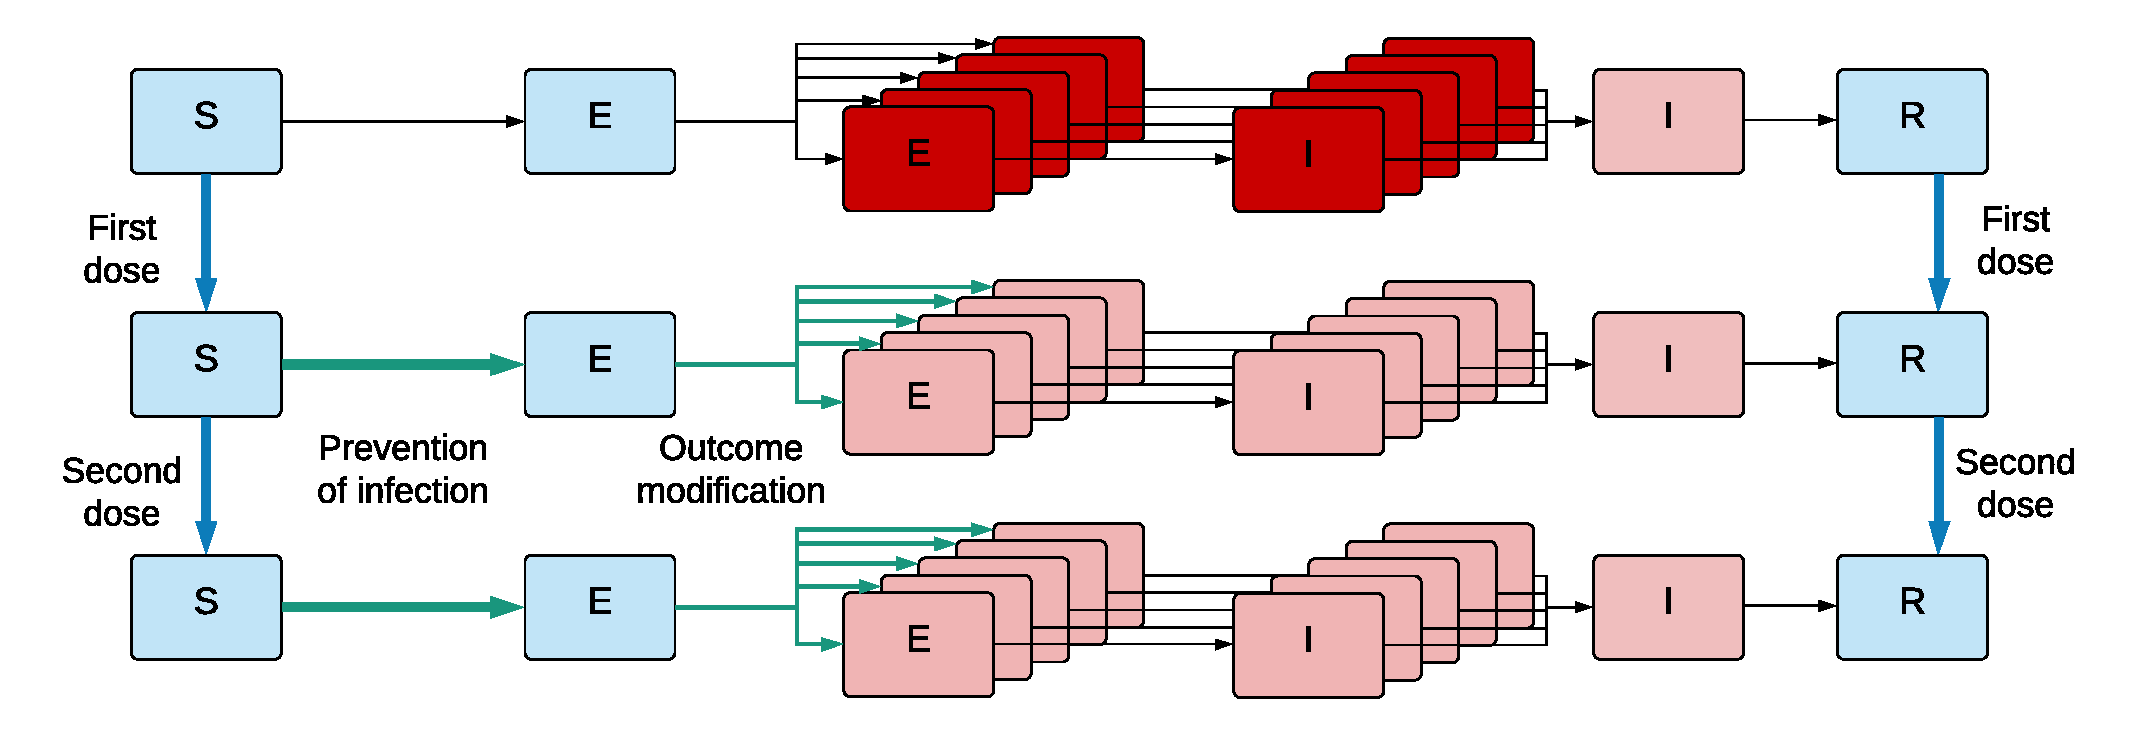
\includegraphics[width=\textwidth]{../covid_19/projects/victoria/victoria_2021/covid_19_vaccination.pdf}
   \title{Unstratified compartmental model structure.}
    \caption{\textbf{Approach to model stratification for vaccination.} Vaccination has three modelled effects: prevention of infection, reduction in severe outcomes given infection and reduction in infectiousness.}
    \label{fig:vaccination}
\end{figure}

\section{Case detection and isolation} \label{cdr}

\subsection{Determining the proportion of cases detected}
We calculate a time-varying case detection rate, being the proportion of all symptomatic cases (clinical strata 2 to 5) that are detected (clinical strata 3 to 5). This proportion is informed by the number of tests performed using the following formula:

\[CDR(time)=1-e^{-shape \times tests(time)}\]

\textit{time} is the time in days from the 31\textsuperscript{st} December 2019 and \textit{tests(time)} is the number of tests per capita done on that date. To determine the value of the shape parameter, we solve this equation based on the assumption that a certain daily testing rate \textit{tests(t)} is associated with a certain \textit{CDR(t)}. Solving for \textit{shape} yields:

\[shape = \frac{-log(1 - CDR(t))}{tests(t)}\]

That is, if it is assumed that a certain daily per capita testing rate is associated with a certain proportion of symptomatic cases detected, we can determine \textit{shape}.
As this relationship is not well understood and unlikely to be consistent across all settings, we vary the \textit{CDR} that is associated with a certain per capita testing rate during uncertainty/calibration.
Given that the \textit{CDR} value can be varied widely, the purpose of this is to incorporate changes in the case detection rate that reflect the empirical historical profile of changes in testing capacity over time.

The proportion of persons entering clinical stratum 3 is calculated once the \textit{CDR} is known, along with the proportion of all incident cases hospitalised (strata 4 and 5).

\subsection{Isolation of detected cases}
As described in the Section \ref{clin} above, as infected persons progress from the early to the late stage of active COVID-19, infectious is reduced for those in the detected strata (3 to 5) to reflect case isolation.

\section{Contact tracing and quarantine}

\subsection{Model adaptation}
We simulate quarantining of persons identified as first degree contacts of COVID-19 patients explicitly through stratification of the compartments representing active COVID-19.
That is, the compartments representing both phases of the incubation period and both phases of active COVID-19 are duplicated are stratified, with model strata referred to as ``traced" and ``untraced".
In model initialisation, all infectious seed is assigned to the untraced stratum.
All newly infected persons commence their incubation period in the untraced stratum of the early incubation period.
As for isolated and hospitalised patients, those undergoing quarantine have their infectiousness reduced by 80\%.

\subsection{Contact tracing process}
Identification of infected persons through contact tracing is assumed to apply to those in their early incubation period, with flows added to the model that transition persons during their incubation period from the untraced to the traced stratum of this compartment type.
The rate of transition from the untraced to the traced stratum of the early incubation period is determined by the proportion of contacts traced.
It is assumed that only the contacts of identified cases can be traced, such that the case detection rate (the proportion of symptomatic cases detected) is considered the ceiling for the proportion of contacts traced.
The proportion of contacts of identified cases that is traced is multiplied by the proportion of contacts whose index is detected (the case detection rate) to determine the proportion of all persons entering the incubation period who are traced.
The proportion of contacts with detected index is calculated as the relative contribution of ever-detected infectious individuals to the total force of infection, given as:

\[ \frac
{\sum_{c \in \mathcal{C}} \sum_{s \in \mathcal{D}} \, prev_{c, s}(t) \times inf_{c, s}}
{\sum_{c \in \mathcal{C}} \sum_{s \in \mathcal{S}} \, prev_{c, s}(t) \times inf_{c, s}} \, ,
\]

where $\mathcal{C}$ is the set of infectious compartments, $\mathcal{S}$ represents all clinical strata and $\mathcal{D} \subset \mathcal{S}$ is the list of detected clinical strata.
The prevalence of infectious compartment $c$ in clinical stratum $s$ at time $t$ is represented by $prev_{c, s}(t)$, and $inf_{c, s}$ is the relative infectiousness of compartment $c$ in clinical stratum $s$.

The proportion of contacts of identified cases traced is considered to decrease as the severity of the COVID-19 epidemic increases, because we expect contact tracing to decline in efficiency as more cases are identified.
That is, we assume that contact tracing is universal as COVID-19 prevalence approaches zero and declines exponentially with increasing prevalence.
The relationship between the proportion of contacts of identified patients who are quarantined and prevalence is given as:

\[q = e^{-prev \times \tau }\]

such that \(e^{-prev \times \tau} \times CDR(t) \) represents the proportion of all contacts of COVID-19 who are quarantined.

Rather than estimate \(\tau\) directly, we estimate the more intuitive quantity of the proportion of contacts of identified patients who would be quarantined at a particular prevalence.
Solving for the previous equation for \(\tau\), we obtain:

\[\tau = \frac{-log(q)}{prev} \]

or \(\tau = \frac{-log(q_{0})}{prev_{0}} \) at a specific prevalence that accords with a particular value of \(q\). Fixing \(prev_{0}\) at \(10^{-3}\), we can vary \(q_{0}\) in calibration as the proportion of contacts of identified cases detected at a prevalence of one active case per thousand population.

\section{Simulation of local NPI implementation during Victoria's second wave}

\subsection{School closures}
The effect of Victorian school closures is captured through the timeline presented in Table \ref{tab:school_timeline}.


\begin{table}[ht]
\renewcommand{\baselinestretch}{1}
	\begin{tabular}[ht]{| p{4.2cm} | p{6.2cm} | p{3.2cm} |}
	\hline
		Date of change & Policy change & Modification applied to school contacts contribution to mixing matrix, \(s(t)\) \\
		\hline
		From model start & Onsite learning & 1 \\
		\hline
		16\textsuperscript{th} July & Schools close for lockdown 5 & 0.1 \\
		\hline
		27\textsuperscript{th} July & Schools re-open after lockdown 5 & 1 \\
		\hline
		5\textsuperscript{th} August & Schools close for lockdown 6 & 0.1 \\
		\hline
		18\textsuperscript{th} September & Four of 13 year levels (foundation to year 2 and year 12) return in regional Vic & 0.30769 (regional only) \\
		\hline
    \end{tabular}
    \title{Timeline used to implement Victorian school closure policies.}
    \caption{\textbf{Timeline used to implement Victorian school closure policies.} The function is applied to both metropolitan and regional services.}
    \label{tab:school_timeline}
\end{table}

\subsection{Macrodistancing in workplaces and other locations}
The functions applied here are determined by the Google mobility data according to Table \ref{tab:mobility_map}, as described above, but are applied separately for each health service. Because Google mobility data pertain to local government areas (LGAs), whereas health service clusters may receive patients from across the state, it was necessary to map mobility data to services. Health service clusters' overall mobility values in each location were calculated using a weighted average of LGA mobility values according to the historical pattern of the origin of patients presenting to services within each service.

As a hypothetical example, if 50\% of patients historically presenting to Barwon South West health services come from the City of Geelong, the mobility data for the City of Geelong will contribute 50\% of the Google mobility estimate of Barwon South West.

Historical patterns of patient presentations by health service cluster were provided by the Victorian Department of Health and Human Services (DHHS).

\subsection{Microdistancing approach}
In this application to Victoria, the microdistancing function \(m(t)\) is comprised of two components: physical distancing and face coverings. Both physical distancing and face coverings micro-distancing are applied to the three non-household locations, such that the microdistancing function for non-household locations is given by: \[m(t)=d(t)^2\times f(t)^2\]
The two interventions are assumed to be independent and so are multiplicative. As for the macrodistancing functions, the two functions of time are squared to represent their effects on both the infector and the infectee in any potentially infectious interaction.
The face covering and physical distancing functions applied for Victoria in this current analysis remain under development and have been replaced by constant functions.



\section{Parameters}
\subsection{Non-age-structured parameters}
This section currently remains under development.
\subsection{Age-specific parameters}

\begin{table}[ht]
\renewcommand{\baselinestretch}{1}
    \begin{tabular}[ht]{| p{2cm} | p{2.5cm} | p{3cm} | p{3cm} | p{2.5cm}|}
    \hline
        Age group (years) & Clinical fraction\textsuperscript{a} & Relative susceptibility to infection & Infection fatality rate & Proportion of symptomatic patients hospitalised \\
        \hline
        0 to 4 & 0.29 & 0.36 & 3 $\times$ 10\textsuperscript{-5} & 0.0777 \\
        \hline
        5 to 9 & 0.29 & 0.36 & 1 $\times$\textsuperscript{-5} & 0.0069 \\
        \hline
        10 to 14 & 0.21 & 0.36 & 1 $\times$\textsuperscript{-5} & 0.0034 \\
        \hline
        15 to 19 & 0.21 & 1 & 3 $\times$\textsuperscript{-5} & 0.0051 \\
        \hline
        20 to 24 & 0.27 & 1 & 6 $\times$\textsuperscript{-5} & 0.0068 \\
        \hline
        25 to 29 & 0.27 & 1 & 1.3 $\times$\textsuperscript{-4} & 0.0080 \\
        \hline
        30 to 34 & 0.33 & 1 & 2.4 $\times$\textsuperscript{-4} & 0.0124 \\
        \hline
        35 to 39 & 0.33 & 1 & 4.0 $\times$\textsuperscript{-4} & 0.0129 \\
        \hline
        40 to 44 & 0.40 & 1 & 7.5 $\times$\textsuperscript{-4} & 0.0190 \\
        \hline
        45 to 49 & 0.40 & 1 & 1.21 $\times$\textsuperscript{-3} & 0.0331 \\
        \hline
        50 to 54 & 0.49 & 1 & 2.07 $\times$\textsuperscript{-3} & 0.0383 \\
        \hline
        55 to 59 & 0.49 & 1 & 3.23 $\times$\textsuperscript{-3} & 0.0579 \\
        \hline
        60 to 64 & 0.63 & 1 & 4.56 $\times$\textsuperscript{-3} & 0.0617 \\
        \hline
        65 to 69 & 0.63 & 1.41 & 1.075 $\times$\textsuperscript{-2} & 0.1030 \\
        \hline
        70 to 74 & 0.69 & 1.41 & 1.674 $\times$\textsuperscript{-2} & 0.1072 \\
        \hline
        75 and above & 0.69 & 1.41 & 5.748 $\times$\textsuperscript{-2, b} & 0.0703 \\
        \hline
        Source/ rationale & 
        Model fitting to age-distribution of early cases in China, Italy, Japan, Singapore, South Korea and Canada taken from upper-left panel of Figure 2b of \cite{RN33}. & Conversion of odds ratios presented in Table S15 of Zhang et al. 2020 to relative risks using data presented in Table S14 of the same study \cite{RN7}.\textsuperscript{c} & Estimated from pooled analysis of data from 45 countries from Table S3 of O'Driscoll et al \cite{RN6}. Values consistent with previous estimates using serosurveys performed in Spain \cite{RN21}. &
        Estimates from the Netherlands as the first wave of infections declined from 4th May to 21st July \cite{RN9}.\\
        \hline        
    \end{tabular}
\end{table}


\section{Calibration}

We calibrated the model using the adaptive Metropolis algorithm described by Haario et al. \cite{RN4}. A standard Metropolis algorithm with fixed proposal distribution parameters was used for the first 500 iterations to initiate the covariance matrix before the adaptive algorithm commenced.

\subsection{Rationale for cluster-specific targets}
For all clusters (both metropolitan and regional), we included the time series of daily notifications for that cluster as a calibration target, using a normal distribution for the likelihood function. A normal distribution is preferred because the mapping process for the notifications for each cluster results in these quantities not being integer-valued.

In addition, we include time series for the following quantities at the state level. Because these quantities are counts, Poisson distributions are used in likelihood calculations:
\begin{itemize}
    \item Daily new COVID-19 notifications
    \item Daily new hospital admissions
    \item Daily new ICU admissions
    \item Daily deaths
\end{itemize}

\subsection{Assigning targets to clusters}
Hospital admissions and ICU admissions can be mapped directly to a health service cluster. Health service clusters include all health care (including public hospitals, private, rehab, acute, mental health, etc.) and some metropolitan services have changed cluster assignment over the years. Mapping was performed as at August 2020.  However, for the other two indicators used (notifications and deaths), mapping was not possible because these events do not necessarily occur within a health service cluster. Therefore, the local government area (LGA) of residence of the person notified or dying is considered. Each notification and death is split proportionately across the health service clusters to which they would typically present, according to historical data on hospital presentations for each LGA provided by DHHS. (Note that only notifications are considered as calibration targets, although these considerations are relevant to the comparison between data and modelled outputs undertaken for validation purposes.)

\subsection{Variation of age-specific proportion parameters using ``adjuster" parameters}
Our parameters included age-specific parameters that were varied up and down together during calibration. These proportion parameters are modified through ``adjuster" parameters that are not strictly multipliers, but are rather implemented in such a way as to scale the base parameter value while ensuring that the adjusted parameter remains a proportion (with range zero to one). In each of these cases, the adjuster parameters can be considered as multiplicative factors that are applied to the odds ratio that is equivalent to the baseline proportion to be adjusted. Specifically, the adjusted proportion is equal to:
\[\frac{proportion \times adjuster}{proportion \times (adjuster-1)+1}\]
This approach was applied for the age-specific fraction hospitalised and the age-specific fraction of active cases symptomatic.

\subsection{Variation of the proportion of patients symptomatic}
The modelled proportion of patients symptomatic differs by age group. However, given that this quantity remains highly uncertain and may vary between settings, it is varied during calibration. A single adjuster is used to increase or decrease each value for each age group.

\subsection{Variation of the proportion of patients hospitalised}
The modelled proportion of patients hospitalised similarly differs by age group, and is also likely to vary between settings. A single adjuster is used to increase or decrease each value for each age group.

\subsection{\hl{Variation of infection fatality rate}}

The infection fatality rate can be defined as the risk of death given an episode of infection, including asymptomatic and undetected episodes. This is considered a more stable quantity than the case fatality rate. However, it is still likely to vary considerably between settings and so is adjusted during the calibration process. Because the epidemic in Victoria was characterised by high rates of transmission and disease in aged care, we fix the infection fatality rate for all age groups up to 74 years to the estimates derived from the literature, but vary the infection fatality rate for those aged 75 and above. This is intended to capture the increased risk of death for those in residential aged care during the second wave, the large majority of whom would be included in this age bracket.

\section{Likelihood function}

Likelihood functions are derived from comparing model outputs to target data at each time point nominated for calibration.

The composite likelihood function is given formally as:
\[\prod_{t}{n_{t}(\theta)d_{t}(\theta)h_{t}(\theta)i_{t}(\theta)} \times \prod_{t,g}{n_{t,g}(\theta,\sigma)}\]
where \(_{t}\) indexes the date, \(_{g}\) indexes the cluster, \(n_{t}\) refers to daily new notifications, \(d_{t}\) to daily deaths, \(h_{t}\) to daily new hospitalisations and \(i_{t}\) to daily new ICU admissions. Each state-wide component uses a Poisson distribution (e.g. \(n_{t}(\theta)=Poiss(\nu_{t}(\theta))\), where \(\nu_{t}(\theta)\) is the number of notifications simulated by the model at date \(t\) under parameter set \(\theta\)), whereas each \(n_{t,g}\) uses a normal likelihood distribution (because these targets are not integer-valued). \(\sigma\) is the ratio of the peak of each cluster-specific notification to the corresponding standard deviation of each of the normal distributions used in calculating their contribution to the likelihood. This was included as a calibration parameter to improve calibration efficiency.
\section{Ordinary differential equations}

For the clearest description of the model, we refer the reader to our code repository, because our object-oriented approach to software development is intended to be highly transparent and readable. For those who prefer dynamical systems such as those presented in the form of ordinary differential equations, we present the following.

    
    \[\frac{dS_{a}}{dt}=-\lambda_{a}(t)\times\sigma_{a}\times S_{a}\]
    \[\frac{dE_{a}}{dt}=\lambda_{a}(t)\times\sigma_{a}\times S_{a}-\alpha E_{a}\]
    \[\frac{dP_{a,c}}{dt}=p_{a,c}(t)\times \alpha E_{a}-\nu P_{a,c}\]
    \[\frac{dI_{a,c}}{dt}=\nu P_{a,c}-\gamma_{c}I_{a,c}\]
    \[\frac{dL_{a,c}}{dt}=\gamma_{c}I_{a,c}-\delta_{a,c}L_{a,c}-\mu_{a,c}L_{a,c}\]
    \[\frac{dR_{a}}{dt}=\sum_{c}{}\delta_{a,c}L_{a,c}\]
    where
    \[\lambda_{a}=\beta\left[\sum_{j,c}\frac{\epsilon\times P_{j}}{N_{j}}\times C_{a,j}(t)+\sum_{j,c}\frac{I_{j,c}\times\iota_{c}+L_{j,c}\times\kappa_{c}}{N_{j}}\times C_{a,j}(t)\right]\]
    \[\sum_{c}p_{a,c}(t)=1,\forall t\in\mathbb{R}\]
    \[\textbf{C}_{0}=\textbf{C}_{H}+\textbf{C}_{S}+\textbf{C}_{W}+\textbf{C}_{L}\]
    \[\textbf{C}(t)=h(t)\times\textbf{C}_{H}+s(t)\times\textbf{C}_{S}+w(t)\times\textbf{C}_{W}+l(t)\times\textbf{C}_{L}\]
    \[l(t)=\frac{re(t)+gr(t)+pa(t)+tr(t)}{4}\]

\section{Calculation of outputs}

\subsection{Incidence}
Incidence is calculated as any transitions into the early active compartment (\textit{``I"}).

\subsection{Hospital occupancy}
Hospitalisation numbers are not reported in the case of Sri Lanka, because the approach to hospitalisation in the country differ considerably from that adopted in the other countries to which the AuTuMN model is applied. Therefore, our approach to simulating hospitalisations is not applicable to Sri Lanka.

\subsection{ICU occupancy}
This is calculated as all persons in the late active compartment in clinical stratum 5.

\subsection{Seropositive proportion}
This is calculated as the proportion of the population in the recovered (\textit{``R"}) compartment. Although very similar numerically to the attack rate, persons who died of COVID-19 are not included in the denominator.

\subsection{COVID-19-related mortality}
This is calculated as all transitions representing death, exiting the model. This is implemented as depletion of the late active compartment.

\subsection{Notifications}
Local case notifications are calculated as transitions from the early to the late active compartment for clinical strata 3 to 5.

\clearpage
\section{Supplemental figures and tables to main text}

\begin{figure}[ht]

    \includegraphics[width=\textwidth]{../covid_19/projects/sri_lanka/supplementary figures/posterior_distributions.png}
    \textbf{\caption{Histograms of prior (blue lines) and posterior (red bars) distributions for epidemiological parameters for Sri Lanka. In the VoC emergence start time the lower bounds and upper bounds for Alpha and Delta strains correspond to, 29th Jan 2021 to 28th Feb 2021 and 04th May 2021 to 03rd July 2021, respectively.}}
    \label{fig:posterior_distributions}
\end{figure}

\begin{figure}[ht]

    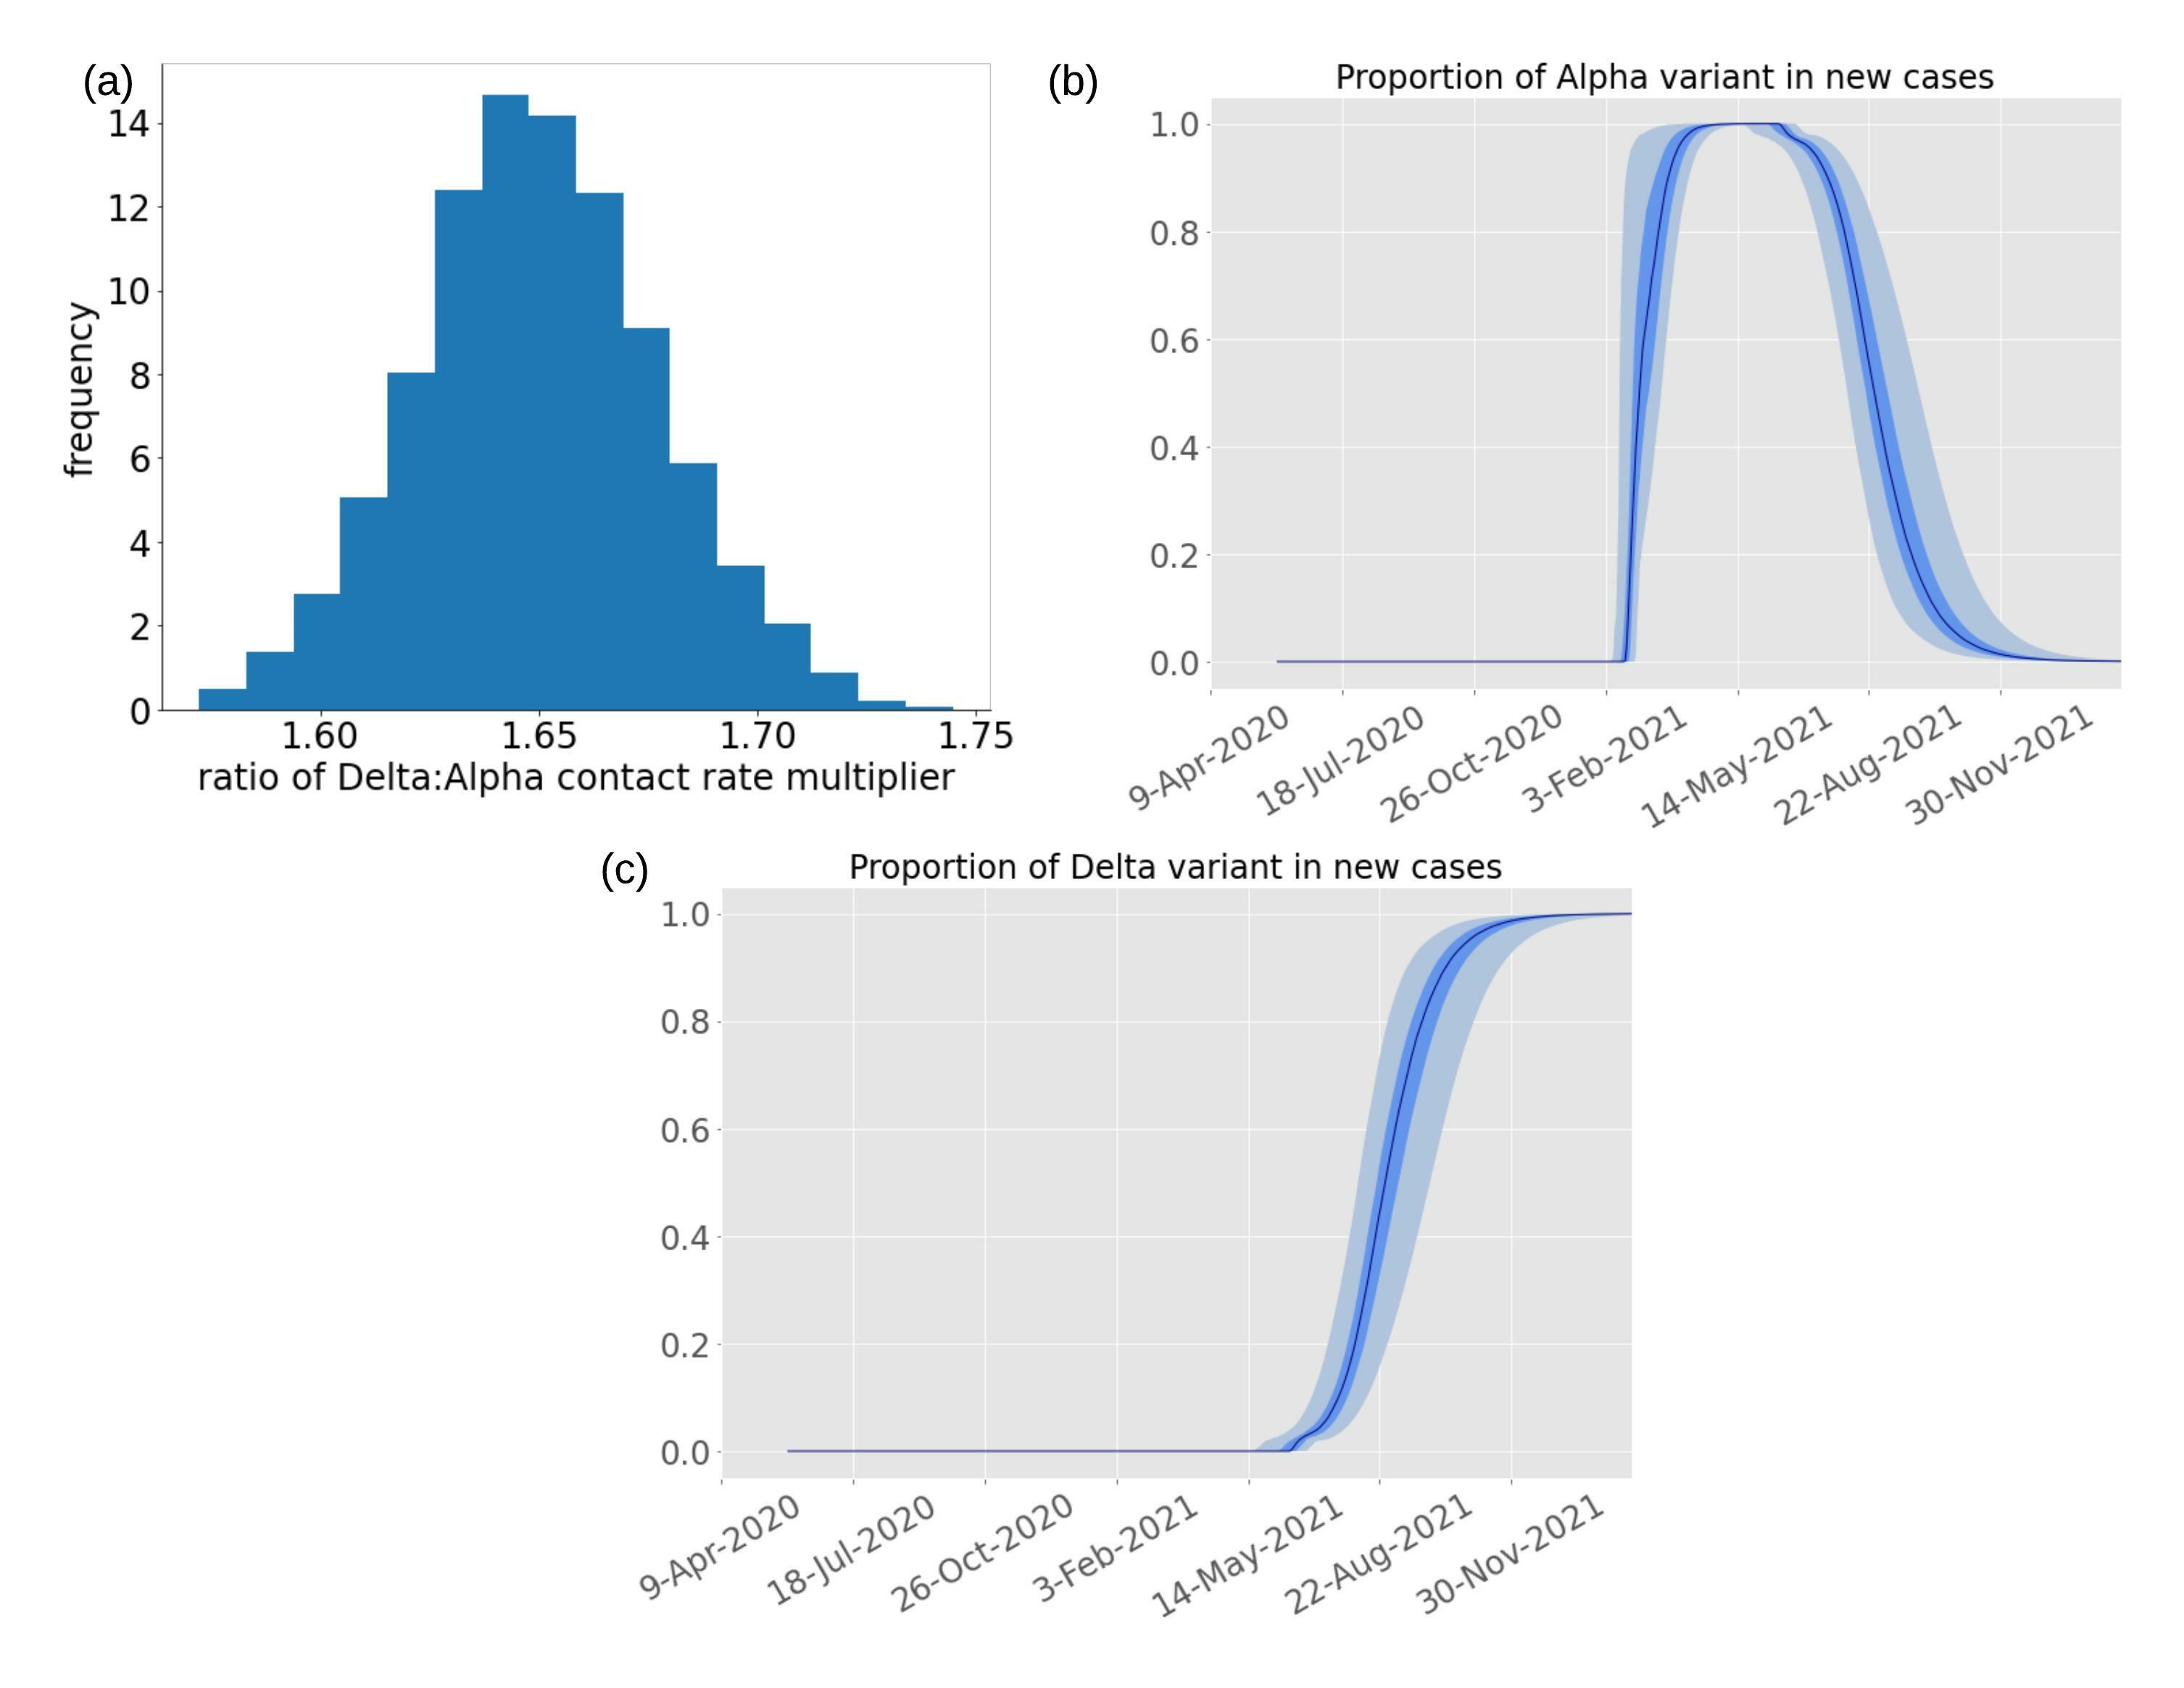
\includegraphics[width=\textwidth]{../covid_19/projects/sri_lanka/supplementary figures/Alpha_Delta.jpeg}
    \textbf{\caption{The ratio of the increased transmissibility of Delta strain to the increased transmissibility of Alpha strain (a), the proportion of Alpha (b) and Delta (c) variants in new cases.}}
    \label{fig:alpha_delta}
\end{figure}

\begin{figure}[ht]

    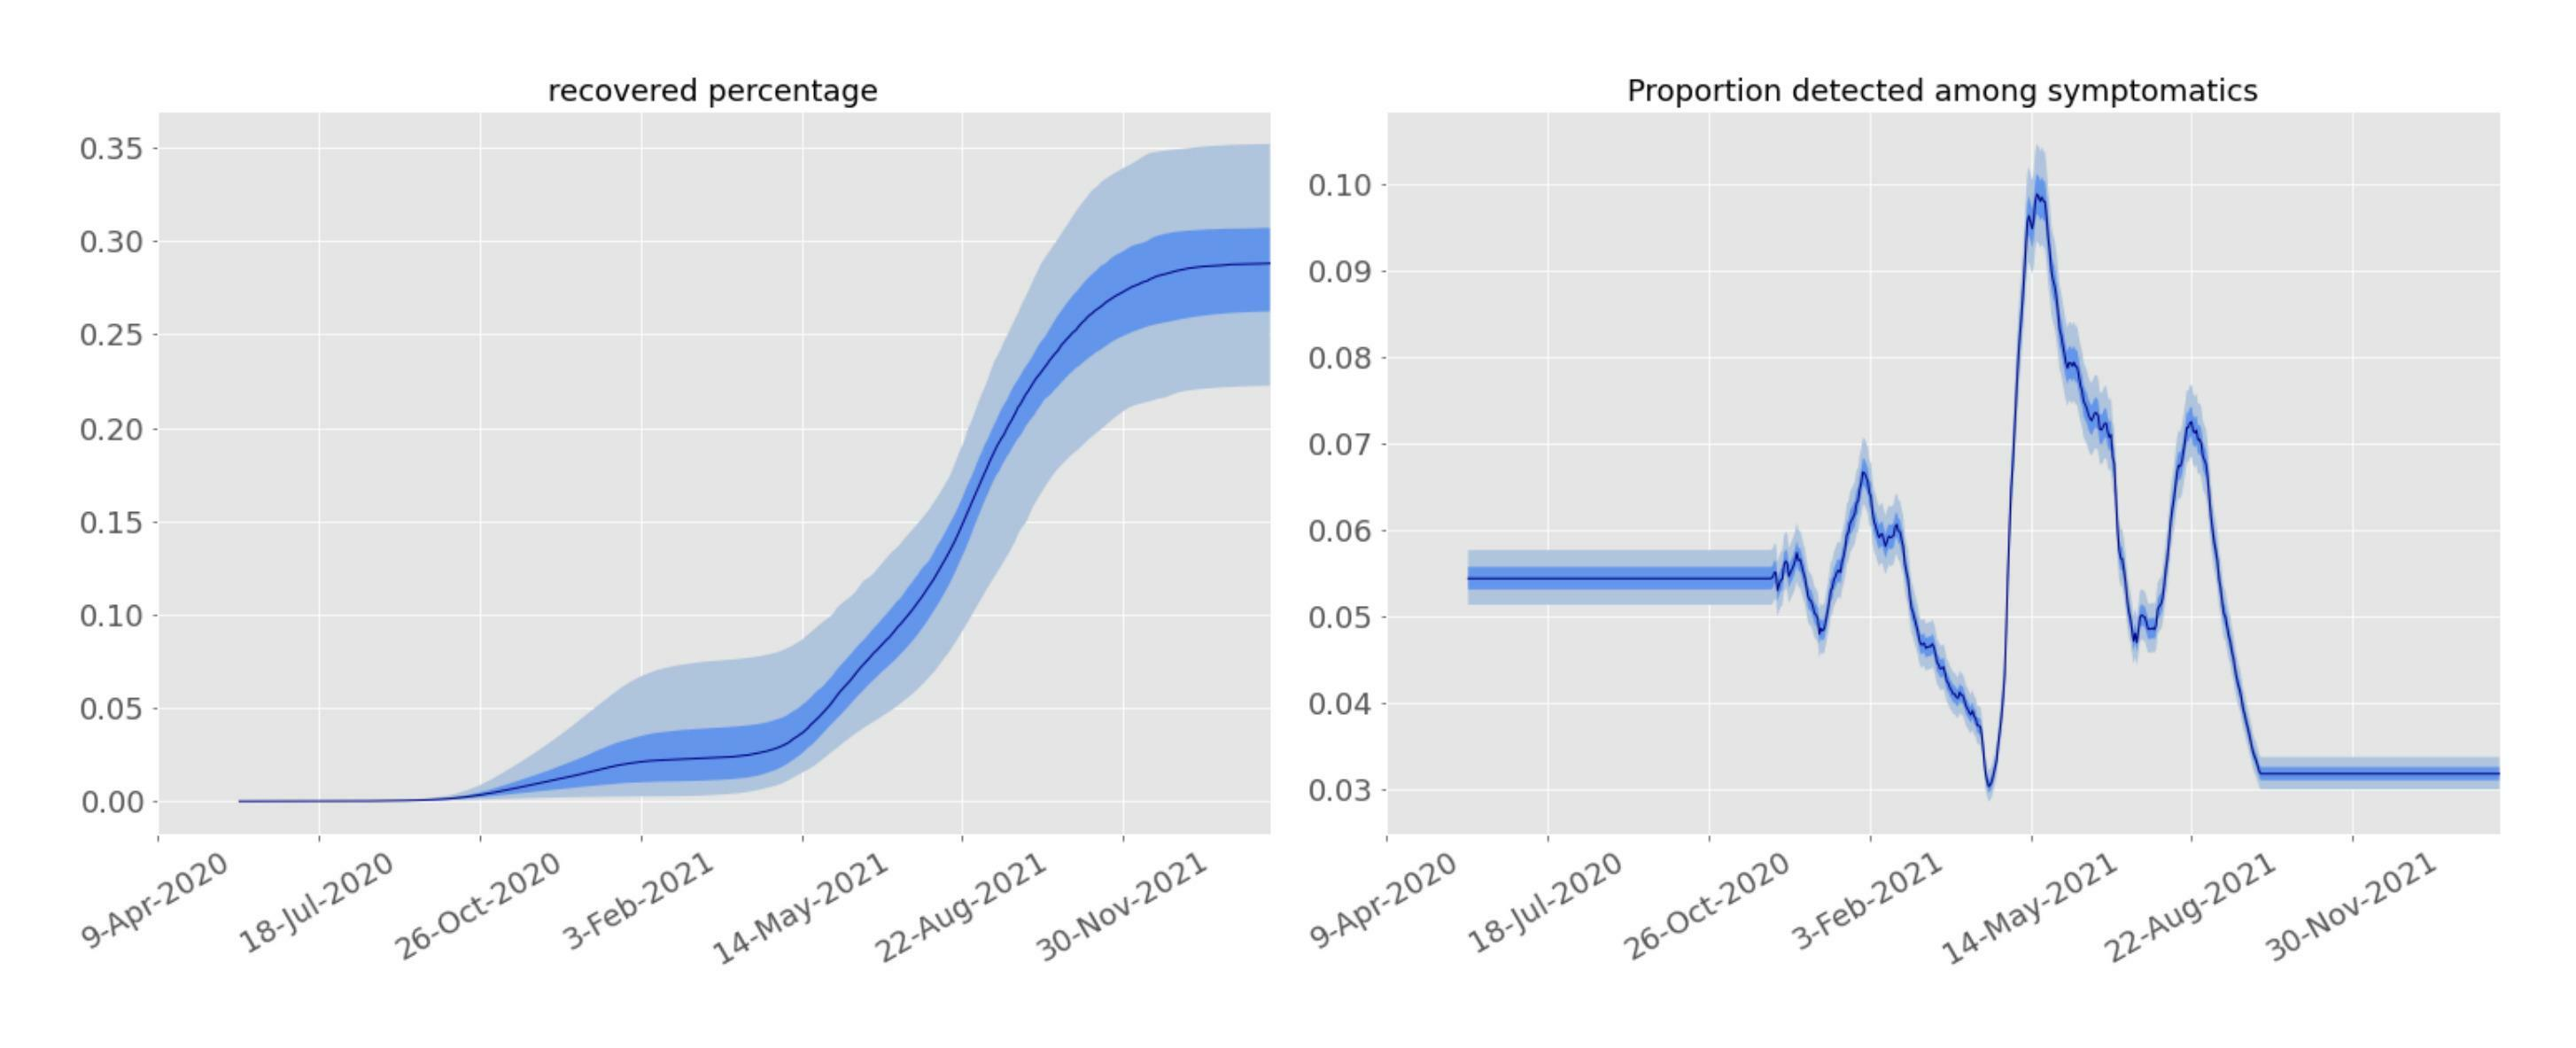
\includegraphics[width=\textwidth]{../covid_19/projects/sri_lanka/supplementary figures/covid_19 - CDR.jpeg}
    \textbf{\caption{The modelled recovered percentage (a) and the model estimated proportion of symptomatic cases (b).}}
    \label{fig:cdr}
\end{figure}
\clearpage
\bibliography{covid_library.bib}
\end{document}
